\input{configuration}

\title{Lecture 15 --- Multilevel Index: B$^{+}$ Trees }

\author{Jeff Zarnett \\ \small \texttt{jzarnett@uwaterloo.ca}}
\institute{Department of Electrical and Computer Engineering \\
  University of Waterloo}
\date{\today}


\begin{document}

\begin{frame}
  \titlepage

 \end{frame}



\begin{frame}
\frametitle{Multilevel Index: B$^{+}$ Trees}

If instead of having just a flat index file, we decide to have multiple levels? 

Then it means instead of performing a simple binary search on the index, we must traverse a tree. 

\begin{center}
	
\includegraphics[width=0.3\textwidth]{images/toomuchwork.jpg}
\end{center}

 \end{frame}



\begin{frame}
\frametitle{Multilevel Index: B$^{+}$ Trees}

At first that may appear counterproductive, or at least, not helpful, since we would still have to traverse a bunch of blocks to get to the item we want to find. 

That is true if we pick a binary tree, but, as the title of this section gives away, that's not what we will do.

\end{frame}


\begin{frame}
\frametitle{Multilevel Index: B$^{+}$ Trees}

Thinking back on how linear search works, we check an item to see if it matches and we reduce the remaining space to check by 1. 

Not efficient. 

\begin{center}
	
\includegraphics[width=0.4\textwidth]{images/84years.jpg}
\end{center}

\end{frame}


\begin{frame}
\frametitle{Multilevel Index: B$^{+}$ Trees}

If we do a binary search, we reduce the remaining space to check by half of its current size. 

Much better. 

Hypothetically we could improve on that if we could reduce the remaining space to search by more than that. 


\end{frame}

\begin{frame}
\frametitle{Fan Out}

This is called the \alert{fan out} of the multilevel index. 

Instead of dividing the remaining space to search by 2 like in binary search, we divide it $n$-ways where $n$ is the fan out. 

Then we reduce the record space by a lot.

\end{frame}

\begin{frame}
\frametitle{Fan Out}

This is called the \alert{fan out} of the multilevel index. 

Searching the multi-level index requires about $log_{fo}($ number of blocks $)$. 

We would like to see the fan out is in the order of 50 - 200.


\end{frame}

\begin{frame}
\frametitle{Fan Out}

If our fan out is five, for example, when we need to find some data then it means we can at each step eliminate 80\% of the remaining search space.

This pattern can be repeated at multiple levels of the index, which allows us to narrow in on the target quickly.

\begin{center}
	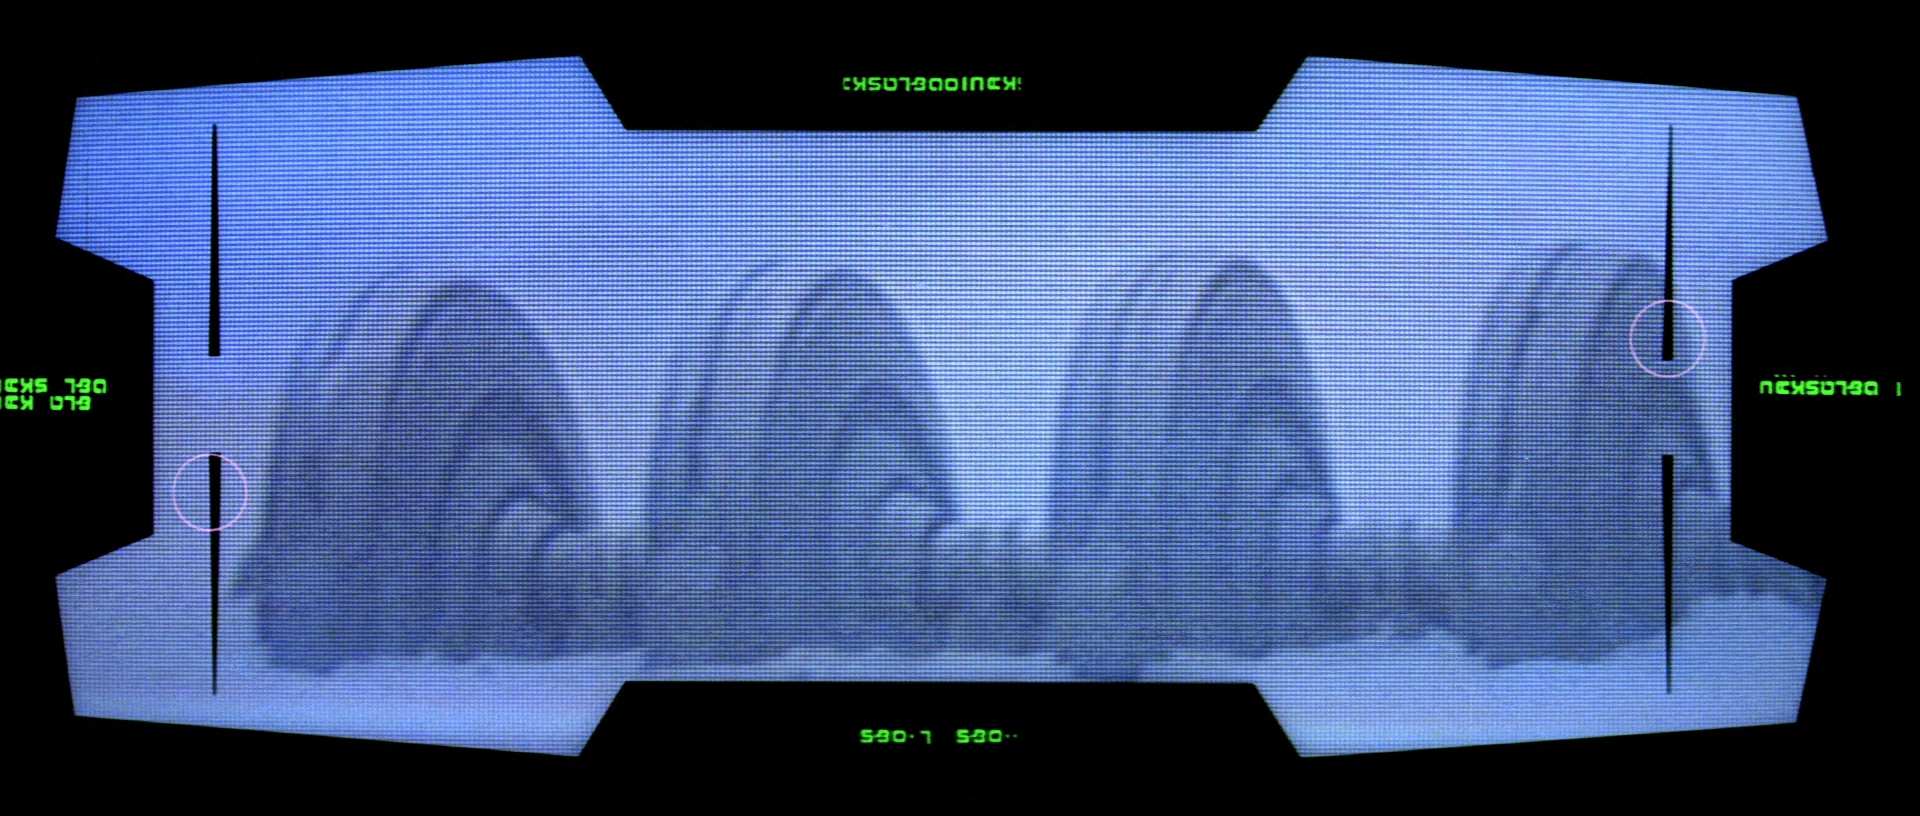
\includegraphics[width=0.75\textwidth]{images/shield-generator.jpg}
\end{center}

\end{frame}

\begin{frame}
\frametitle{ISAM}

A common file organization is called ISAM -- Indexed Sequential Access Method. 

The IBM version of this has a two level index which maps as closely as possible to the hard drive underlying structure. 

MySQL has its own implementation called MyISAM but it is terrible...\\
\quad Please do not use it; use InnoDB instead. 

\end{frame}

\begin{frame}
\frametitle{Multilevel Index}
Let us examine a very simple approach for multi-level indexing. 

\begin{center}
	
\includegraphics[width=0.5\textwidth]{images/happenedbefore.jpg}
\end{center}


The lowest level consists of blocks that contain pointers to the second level. 

The second level has blocks that contain pointers to the actual file. 



\end{frame}

\begin{frame}
\frametitle{Multilevel Index}
Whether the file has multilevel index or not, in an index sequential file the performance does get slower as more entries are added. 

Reorganization can help, but it is expensive. Instead we might wish to use a balanced tree structure, specifically, a B$^{+}$ tree.


\end{frame}

\begin{frame}
\frametitle{B$^{+}$ Tree Refresher}

A B$^{+}$ Tree structure, formally, has the following characteristics:

\begin{enumerate}
	\item The tree is made up of nodes (have children) and leaves (have no children).
	\item Each node contains at least one key identifying a file record, and more than one pointer to child nodes or child leaves.
	\item Each node has some maximum number of keys.
	\item The keys in a node are stored in non-decreasing order.
\end{enumerate}

\end{frame}

\begin{frame}
\frametitle{B$^{+}$ Tree Refresher}

And a B$^{+}$ Tree of degree $d$ has the following properties:

\begin{enumerate}
	\item Every node has at most $2d-1$ keys and $2d$ children ($2d$ pointers).
	\item Every node other than the root has at least $d-1$ keys and $d$ pointers. Each internal node except the root is at least half full and has at least $d$ children.
	\item All leaves appear on the same level.
	\item A non-leaf node with $k$ pointers contains $k-1$ keys.
\end{enumerate}


\end{frame}


\begin{frame}
\frametitle{B$^{+}$ Tree Refresher}


To find something in a B$^{+}$ Tree, the general algorithm is fairly simple:

\begin{enumerate}
	\item Start at the root node. 
	\item If the key is in the current node, it is found, and the algorithm terminates.
	\item If the key is less than the smallest key in this node, follow the leftmost pointer; go to step 2.
	\item If the key is greater than the largest key in this node, follow the rightmost pointer; go to step 2.
	\item If the key is between the values of two adjacent keys, follow the pointer between them; go to step 2.
\end{enumerate}


\end{frame}

\begin{frame}
\frametitle{B$^{+}$ Tree Refresher}

Insertion into the B$^{+}$ Tree is more complicated, because of the rules that keep the tree balanced:

\begin{enumerate}
	\item Search the tree for the key. If it is not found, then we are at least looking at the block where it would be if it were there.
	\item If this node has fewer than $2d-1$ keys (that is, it is not full), insert the key into this node in the proper sequence. The algorithm terminates.
	\item If the node is full, split this node around the median key into two new nodes with $d-1$ keys each. Promote the median key to the higher level. If the new node is less than the median key, insert it in the left-hand new node; otherwise into the right.
	\item The promoted node is inserted into the parent node in order, splitting the parent if the parent is already full.
	\item If the process of promotion reaches the root node and the root is full, then splitting and promotion occurs and the height of the tree increases by 1.
\end{enumerate}



\end{frame}

\begin{frame}
\frametitle{B$^{+}$ Tree Refresher}

Deletion is a little bit similar to insertion (but a little bit complicated):

\begin{enumerate}
	\item Search the tree for the key. If it is not found, then there is nothing to do and the algorithm terminates.
	\item Remove the target (and remove it from the parent nodes if it appears at intermediate levels as well), shifting the remaining entries if needed to ensure there are no gaps.
	\item If the current node is the root and there is only one remaining child, then the child is the new root and delete the current node.
	\item Otherwise, if the current node is less than half full then:
		\begin{enumerate}
			\item If the entries in the current node and that of an immediately adjacent node, then coalesce with that adjacent node and update the pointers of the parent.
			\item Otherwise, redistribution is necessary: move an item from the adjacent node so that the current node is at least half full and update the pointers of the parent.
		\end{enumerate}
\end{enumerate}



\end{frame}


\begin{frame}
\frametitle{B+? Why not A+?}

We require that leaf nodes be at least half full (unless it is the root node).

The last pointer in a leaf node chains to the next leaf node to allow relatively quick access if we need to move through the data sequentially. 

So the last pointer is reserved and can't point directly to data. 

\end{frame}


\begin{frame}
\frametitle{B+? Why not A+?}


Non-leaf nodes are sometimes called internal nodes. 

Unlike your typical B-Tree, the items in the non-leaf nodes are duplicates (repeats) of the ones below. 

The pointers in the non-leaf nodes point to leaf nodes, not the actual data.


\end{frame}

\begin{frame}
\frametitle{B$^{+}$ Example}

Assume a node is 4~KB, we are searching a field of length 32 bytes, and pointers to disk blocks are 8 bytes. 

This means we can fit about 100 entries in a block. 

If the file to be queried contains 1 million records, then a lookup requires only $\lceil log_{50}(1~000~000) \rceil = 4$ accesses. 
\end{frame}

\begin{frame}
\frametitle{B$^{+}$ Example}

This is the worst case, though, since the root node may be in the buffer frequently due to its frequent access. 

If we had to do this with a regular binary tree, the $\lceil log_{2}(1~000~000) \rceil = 20$ accesses and that is also the worst case for binary search.


\end{frame}

\begin{frame}
\frametitle{Instructor Relation}

And now let us see an example of applying that to the ``instructor'' relation. First, a leaf node:

\begin{center}
	\includegraphics[width=0.7\textwidth]{images/b-tree-instructor.png}
\end{center}

\end{frame}

\begin{frame}
\frametitle{Instructor Relation}

And then the complete tree for the instructor relation:

\begin{center}
	\includegraphics[width=0.9\textwidth]{images/b-tree-complete}
\end{center}

\end{frame}



\begin{frame}
\frametitle{B-Tree Equivalent}

If this were a regular B-Tree and not a B$^{+}$ Tree then the storage would look something like this

\begin{center}
	\includegraphics[width=0.9\textwidth]{images/b-tree-equivalent}
\end{center}

\end{frame}

\begin{frame}
\frametitle{Small Considerations in Indexing: Strings}

Strings can cause a bit of a small problem when it comes to B$^{+}$ Trees because they can be of variable length or rather long. 

This may cause a pretty ``tall'' tree and lose the benefits of the structure. 

\end{frame}

\begin{frame}
\frametitle{Small Considerations in Indexing: Strings}


The suggested solution is called prefix compression: store a prefix of the search key value that is sufficient to distinguish the sub-trees. 

Thus we could store in a non-leaf node ``Jans'' instead of ``Jansen''. 

The closest two subtrees are under the subtrees are on the left ``Janet'' and on the right ``Janson'' (note different spelling).

\end{frame}

\begin{frame}
\frametitle{Small Considerations in Indexing: File Organization}

Just as we have made use of a B$^{+}$ Tree organization for the index file, the actual file containing records could be stored using B$^{+}$ Trees as well.

\end{frame}


\begin{frame}
\frametitle{Cover Me, I'm Going In!}

A \alert{covering index} is one that stores the value of some attributes (other than things we search on) alongside the pointers to the record. 

This increases the size of the index, but allows us to fulfill some queries without having to even go to the data blocks of the file at all. 

The advantage, of course, is that this can be much faster. 

The downside is that it increases the size of the index, means fewer items can fit in one index block, and requires additional overhead to keep it up to date.


\end{frame}

\begin{frame}
\frametitle{Covering Index}

To give an example, it might be sensible to have in the covering index for employees, their last name alongside the regular index search key (ID). 

This would mean that queries where only the name is required, or name and ID, don't need to go into the file blocks at all.

\end{frame}

\begin{frame}
\frametitle{Multiple Key Indexes}

All discussion so far has covered the simple scenario where one index on one attribute is being used for a query. 

\begin{center}
	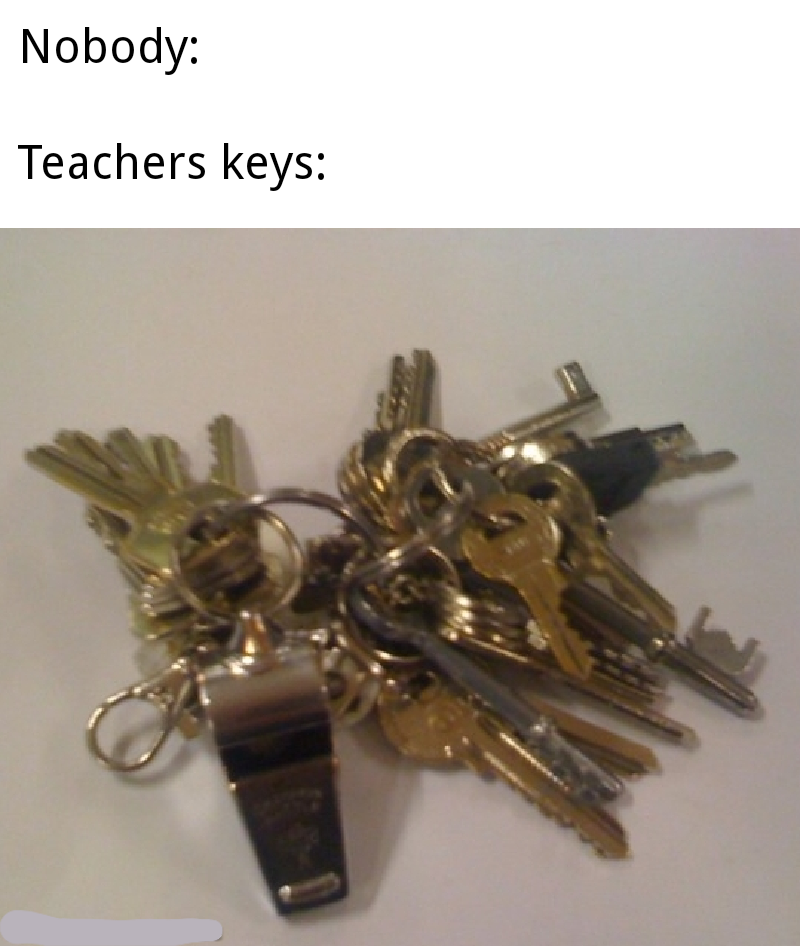
\includegraphics[width=0.3\textwidth]{images/keys.png}
\end{center}

However, that is not the only way. Sometimes an index will be constructed on two attributes, or, we can combine two (or more) indexes on a single attribute. 


\end{frame}

\begin{frame}
\frametitle{Indexes on Multiple Attributes}

Let us imagine that we have a set of addresses. 

It is likely that we may want a composite key on the attributes of (city, province) since city names can be duplicated. 

There is a Waterloo in Ontario and also Quebec (also Belgium...). 

\begin{center}
	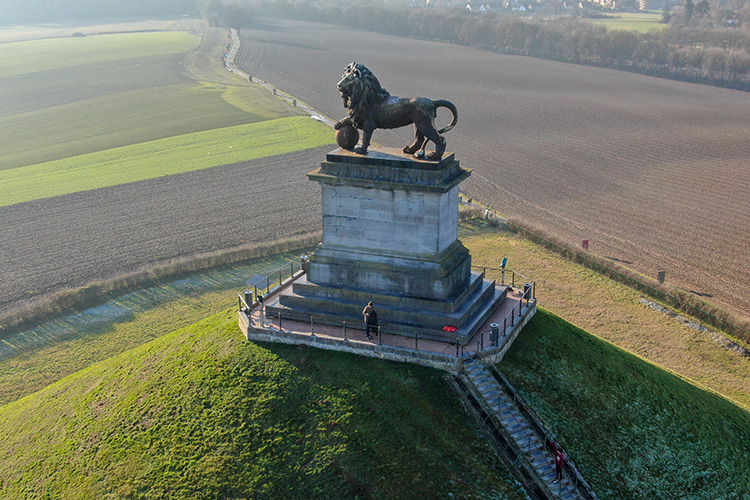
\includegraphics[width=0.4\textwidth]{images/belgium.jpg}
	
\includegraphics[width=0.4\textwidth]{images/sad-napoleon.jpg}
\end{center}


\end{frame}

\begin{frame}
\frametitle{Indexes on Multiple Attributes}

If such an index is defined, then the search key in the tree structures will be the combination of both attributes. 


This is helpful in situations where we know that we are going to search on particular combinations of a certain attribute frequently. 

The city-province example is just one of many where we are likely to perform queries that hit both attributes. 


\end{frame}


\begin{frame}
\frametitle{Indexes on Multiple Attributes}
It may help to think of composite keys as just sort of smashing together the two attributes (perhaps with some separator like a dash).

You end up with Waterloo-ON as the key. 

From there it works mostly like the regular search. 

Assuming there is no index on city alone, if we wanted to find all addresses with the name Waterloo, this is possible. 

Our search term in the tree structure is then something like ``Waterloo-\%''.


\end{frame}

\begin{frame}
\frametitle{Combining Multiple Indexes}

Let us imagine that employees have an index defined on the fields ID, department, and salary. 

We wish to do a select that finds the IDs of all employees with the department name ``development'' and salary above \$100~000. 

How would we do it?

\end{frame}

\begin{frame}
\frametitle{Three Roads to Success}


1. Use the index on the department to find all records for the development department. 

Check each record to see if the salary is above \$100~000.

\end{frame}

\begin{frame}
\frametitle{Three Roads to Success}
2. Use the index on salary to find all records for employees with a salary above \$100 000. 

Check each record to see if the department equals development.

\end{frame}

\begin{frame}
\frametitle{Three Roads to Success}
	3. Use the index on the department to find all records for the development department. 
	
	Use the index on salary to find all records for employees with a salary above \$100 000. 
	
	Compute the intersection of the pointers to find out which ones satisfy both criteria.

\end{frame}

\begin{frame}
\frametitle{Three Roads to Success}

Which approach is best?


\begin{center}
	
\includegraphics[width=0.5\textwidth]{images/threeways.png}
\end{center}

\end{frame}

\begin{frame}
\frametitle{Which Option?}

It depends a lot on our data, but at a first glance only the third option makes use of both indexes, but it does require the computation of the intersection. 

The first approach may be very efficient if the number of employees in the development department is quite small. 

Similarly, the second approach is quite efficient if the number of employees making over \$100~000 is quite small. 

The third approach is perhaps best if neither the department nor the number of people with a large salary is small...

\end{frame}

\begin{frame}
\frametitle{So Confused, So Hard To Choose}

This idea that there are three different ways to carry out the requested operation is actually an interesting and large topic. 

We will therefore take the next few lectures to discuss how the database server understands a query, optimizes it, and carries it out. 


\end{frame}


\end{document}

